%----------------------------------------------------------------------------------------
%	PACKAGES AND OTHER DOCUMENT CONFIGURATIONS
%----------------------------------------------------------------------------------------

\documentclass[paper=a4, fontsize=11pt]{scrartcl} % A4 paper and 11pt font size

% ---- Entrada y salida de texto -----

\usepackage[T1]{fontenc} % Use 8-bit encoding that has 256 glyphs
\usepackage[utf8]{inputenc}
%\usepackage{fourier} % Use the Adobe Utopia font for the document - comment this line to return to the LaTeX default

% ---- Idioma --------

\usepackage[spanish, es-tabla]{babel} % Selecciona el español para palabras introducidas automáticamente, p.ej. "septiembre" en la fecha y especifica que se use la palabra Tabla en vez de Cuadro

% ---- Otros paquetes ----
\usepackage{csquotes} %Para permitir el uso de comillas Quotes https://tex.stackexchange.com/questions/36812/isnt-there-any-other-way-of-doing-double-quotes-in-latex-besides
\usepackage[hyphens]{url} % ,href} %para incluir URLs e hipervínculos dentro del texto (aunque hay que instalar href)
\usepackage{hyperref}
\usepackage{color}
\usepackage{graphics,graphicx, floatrow} %para incluir imágenes y notas en las imágenes
\usepackage{graphics,graphicx, float} %para incluir imágenes y colocarlas
\usepackage{svg}

\graphicspath {{./img/}}

\usepackage{listings}  %para introducir comandos

\lstdefinestyle{mybash}
{basicstyle=\ttfamily,
  showstringspaces=false,
  commentstyle=\color{red},
  keywordstyle=\color{blue},
  language=bash,
  alsoletter=/,
  basicstyle=\footnotesize,
  numbers=left,
  stepnumber=1,
  showstringspaces=false,
  tabsize=1,
  breaklines=true,
  breakatwhitespace=false,
}

\lstdefinestyle{yaml}
{basicstyle=\ttfamily,
  commentstyle=\color{red},
  keywordstyle=\color{blue},
  basicstyle=\color{blue}\footnotesize,
  rulecolor=\color{black},
  string=[s]{'}{'},
  stringstyle=\color{blue},
  comment=[l]{:},
  commentstyle=\color{black},
  morecomment=[l]{-}
  }

\lstdefinestyle{mysql}
{basicstyle=\ttfamily,
  showstringspaces=false,
  commentstyle=\color{red},
  keywordstyle=\color{blue},
  language=sql,
  basicstyle=\footnotesize,
  numbers=left,
  stepnumber=1,
  showstringspaces=false,
  tabsize=1,
  breaklines=true,
  breakatwhitespace=false,
}


% Para hacer tablas comlejas
%\usepackage{multirow}
%\usepackage{threeparttable}

%\usepackage{sectsty} % Allows customizing section commands
%\allsectionsfont{\centering \normalfont\scshape} % Make all sections centered, the default font and small caps

\usepackage{fancyhdr} % Custom headers and footers
\pagestyle{fancyplain} % Makes all pages in the document conform to the custom headers and footers
\fancyhead{} % No page header - if you want one, create it in the same way as the footers below
\fancyfoot[L]{} % Empty left footer
\fancyfoot[C]{} % Empty center footer
\fancyfoot[R]{\thepage} % Page numbering for right footer
\renewcommand{\headrulewidth}{0pt} % Remove header underlines
\renewcommand{\footrulewidth}{0pt} % Remove footer underlines
\setlength{\headheight}{13.6pt} % Customize the height of the header

\setlength\parindent{0pt} % Removes all indentation from paragraphs - comment this line for an assignment with lots of text

\newcommand{\horrule}[1]{\rule{\linewidth}{#1}} % Create horizontal rule command with 1 argument of height

%https://es.overleaf.com/learn/latex/Inserting_Images
%Ruta relativa de   imagenes
\graphicspath{ {img/} }

\title{
\normalfont \normalsize

\includegraphics[width=0.4\textwidth]{img/osl.png}~\\[1cm]
\textsc{\textbf{OSL - Oficina de Software Libre \\ 2023 \\ Universidad de Granada} \\ [25pt] }
\horrule{0.5pt} \\[0.4cm] % Thin top horizontal rule
\huge Manual del operador de Clonezilla Server con Ansible. \\ 
\horrule{2pt} \\[0.5cm] % Thick bottom horizontal rule
}

\author{Oficina de Software libre - Pedro A. Mayorgas Parejo} % Nombre y apellidos

\date{\normalsize\today} % Incluye la fecha actual

%----------------------------------------------------------------------------------------
% DOCUMENTO
%----------------------------------------------------------------------------------------

\begin{document}

\maketitle % Muestra el Título

\newpage %inserta un salto de página

\tableofcontents % para generar el índice de contenidos

\newpage

\section{Prefacio}

Este proyecto surge de la necesidad de reducir los tiempos de trabajo físico de clonación de imágenes preparadas para decenas de máquinas en un tiempo corto.
La Oficina de Software Libre, en concreto su personal, ha tenido que responder a una demanda creciente de equipos donados, lo cual constuía un consumo de tiempo elevado
por equipo. Siguiendo la \textbf{Ley de Amdahl}, este proyecto centra su esfuerzo en mejorar los tiempos de trabajo en la parte de clonación y provisionamiento de software.
\vspace{5mm}
\textbf{¿Cuánto de mejora?} Las mejoras han sido de pasar de tener preparados 1 equipo por día hasta un máximo de 16 equipos por día. Un S de 15 o en porcentaje un 150\% de mejora, que se puede conseguir más pero
el personal se satura si tiene que revisar, ampliar, limpiar, reparar, preparar el equipo desde el almacen.

\section{Software Utilizado}

El software utilizado para tal propósito ha sido:

\begin{itemize}
	\item \textbf{Distribución de GNU/Linux:} Debian 11.6
	\item \textbf{Ansible como provisionamiento}.
	\item \textbf{DRBL Stable 2.5.1-16}
\end{itemize}

\subsection{Información de los servicios utilizados: DRBL}

\textbf{DRBL - Diskless Remote Boot Linux}, utiliza un servicio basado en TFTP para enviar las imágenes de clonación a través de sistemas que lo solicitan por PXE. 
Primero ofrece una dirección IPv4 privada por DHCPv4 para identificar al cliente que solicita una clonación, luego ofrece un " GRUB " con distintos campos,
basado el protocolo TFTP, que permite la selección de imágenes NetInstall (No cubiertas por este Manual del Operador), o la imagen precargada para clonación y dicha imagen
se indica en el modo en el que va a funcionar Unicast o Multicast.
\vspace{5mm}
La preferencia de uso de Unicast o Multicast dependerá del operador, pero se deben tener en cuenta los siguientes factores:

\begin{itemize}
	\item Selección de Multicast debe ser en base a los siguientes factores:
	\begin{itemize}
		\item El Switch Físico o la tarjetas de red es un cuello de botella probable, es decir que tiene menos de 1 Gigabit/s.
		\item El HDD utilizado es mecánico y no está en RAID.
		\item Poca memoria RAM para caché de la imagen.
	\end{itemize}

	\item Selección de Unicast debe ser en base a los siguientes factores:

	\begin{itemize}
		\item Los equipos no están disponibles en una cantidad predeterminada para el Multicast. Se quiere sacar en serie de 1 en 1, pero sin pausas en la clonación.
		\item Uso de SSD o un RAID, esto importa ya que el acceso aleatorio a la imagen a clonar no causa esperas o latencias elevadas. Teniendo en cuenta que cuando el nº de equipos por unicast conectados crece y están en momentos distintos de la clonación, 
		estos demandan regiones de datos de la imagen distintos provocando un impacto en los acceso E/S ralentizando los progresos.
		\item Gran cantidad de RAM disponible como caché.
		\item Uso de switch y tarjetas de red de gran capacidad 1Gbit/s.
	\end{itemize}
\end{itemize}

El uso de tarjetas de red de Gigabit es suficiente, ya que los equipos objetivos de la clonación son equipos de hace 10 años o más, por lo que su interfaz 
SATA es la versión I o II (1.5 Gigabits/s o 3 Gigabits/s) que junto a un disco duro mecánico de 5200 RPM, nunca van a poder alcanzar el máximo rendimiento, 
la escritura no pasa de los 130 MBytes/s siempre está limitada por los discos de E/S. Tampoco se ha considerado necesario que el servidor necesite mas capacidad de red, 
por los motivos referidos arriba, el servidor es del orden de 4-5 veces más rápido que la demanda que junto con la caché RAM, apenas le supone una carga real, 
porque las imágenes son servidas como volúmenes de cintas.

Además se debe tener en cuenta la máquina sobre la que se va a instalar el servicio, ya que si esta es UEFI o BIOS, puede generar ciertas incompatibilidades a la hora
de generar una imagen de kernel preparada para las máquinas que lo soliciten por PXE, siendo la mayoría a fecha de 2023 de BIOS legacy.

\newpage
\section{Ansible}

Ansible es una herramienta de provisionamiento que, tiene el objetivo de automatizar tareas que son repetitivas o que requieren de un tiempo pero que ya se han 
realizado en otros servidores. Ansible usa el servicio SSH para la comunicación segura de las directivas de los playbook, por lo que es necesario tener instalado OpenSSH-server en el servidor.
\vspace{5mm}
Se complementa con la herramienta DRBL, debido a que la OSL tiene la necesidad de tener una automatización del despliegue del servicio DRBL, ya que los 
equipos usados para ofrecer dicho servicio varían a lo largo de las campañas de donación debido al espacio o bien por reutilizar los equipos que anteriormente
se usaban como servidor, para otros propósitos que se consideren mas oportunos. Además se intenta ofrecer una automatización atemporal, donde un futuro operador que no conozca 
la herramienta sea capaz de desplegar este servicio sin tener un conocimiento previo o necesidad de una investigación que pueda consumir un tiempo.
\vspace{5mm}
La automatización abarca y resuelve 4 problemas:

\begin{itemize}
	\item \textbf{Problema 1:} Despliegue automatizado del servicio DRBL en un equipo nuevo.
	\begin{itemize}
		\item \textbf{playbook:} deploy\_drbl.yml
	\end{itemize}
	\item \textbf{Problema 2:} Provisionamiento o backup de imágenes de clonación hacia/desde el servidor usando Rsync.
	\begin{itemize}
		\item \textbf{playbook:} provisioning\_ocs.yml
	\end{itemize}
	\item \textbf{Problema 3:} Selección de imágenes de clonación y selección del modo del servidor, esto es Multicast o Unicast.
	\begin{itemize}
		\item \textbf{playbook:} provisioning\_ocs.yml
	\end{itemize}
	\item \textbf{Problema 4:} Redimensión de particiones, sistemas de ficheros, provisionamiento y actualización del software de las imágenes ya clonadas en el equipo de destino.
	\begin{itemize}
		\item \textbf{playbook:} client\_ssh\_proxy/playbook/update\_clients.yml
	\end{itemize}
\end{itemize}

Cada problema tiene un playbook propio menos el 2 y 3, que van en el mismo playbook ya que el provisionamiento de la imagen a veces implica la necesidad de 
querer indicarle al servicio que ofrezca esa imagen para clonar ya.
\vspace{5mm}
La ejecución de los playbooks se indicará en cada sección que explique cada uno de ellos, ya que se incluyen variables que deben ser editadas para poder desplegar el servicio.
\vspace{5mm}
\textbf{Importante:} Cuando creamos una imagen para la clonación debemos tener en cuenta de incluir el servicio OpenSSH Server u otro que nos permita realizar conexiones de SSH, así
como inyectar una clave pública de la workstation desde la que controlamos el proceso para poder utilizar el playbook del problema nº4. También en el servidor DRBL debemos tener
el servicio por supuesto con su clave pública inyectada para que Ansible pueda enviar los comandos de despliegue o provisionamiento a través de una conexión SSH al servidor, así como
permitir usar el servidor de DRBL como un SSH bastión que permita dar un salto a todas las direcciones IPv4 privadas que tengan un lease de DHCP.


Para instalar Ansible debemos ejecutar el siguiente comando:

\begin{lstlisting}[style=mybash]
python3 -m pip install --user ansible
\end{lstlisting}

\begin{figure}[H]
	\centering
	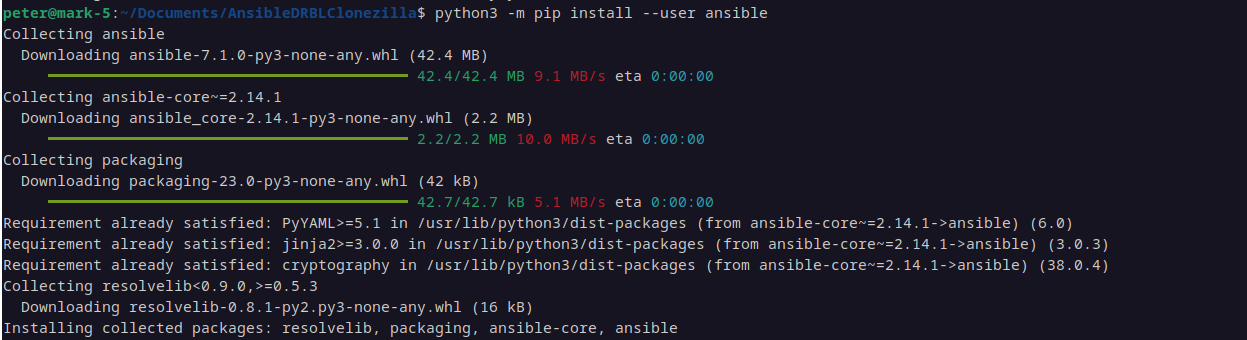
\includegraphics[scale=0.30]{ansible/install-ansible}
	\caption{Proceso de instalación de Ansible.}
\end{figure}

\newpage
\subsection{playbook: deploy\_drbl}

\textbf{Requisitos mínimos para el despliegue del servicio:}
\begin{itemize}
	\item \textbf{CPU:} 2 a 4 cores.
	\item \textbf{RAM:} 8GiB o más. Si se incorpora mas memoria RAM, el sistema la puede utilizar como caché para evitar el acceso a disco, útil cuando queremos el modo UNICAST.
	\item \textbf{NET:} 2 tarjetas de red 1Gbit Ethernet.
\end{itemize}

El servicio DRBL se despliega como el siguiente diagrama, donde podemos visualizar por qué necesitamos 2 tarjetas de red asociadas a la máquina, el motivo principal, es que necesita
una red privada para poder mandar las solicitudes de DHCPv4 a los clientes que quieran utilizar el protocolo PXE para poder arrancar sin disco. Por lo tanto no podemos utilizar 
solamente una tarjeta de red. Además esta configuración que se despliega permite a los clientes cuando hayan terminado de realizar el clonado conectarse a internet por medio de una
NAT preconfigurada por el servicio DRBL que le permita obtener actualizaciones.

\begin{figure}[H]
	\centering
	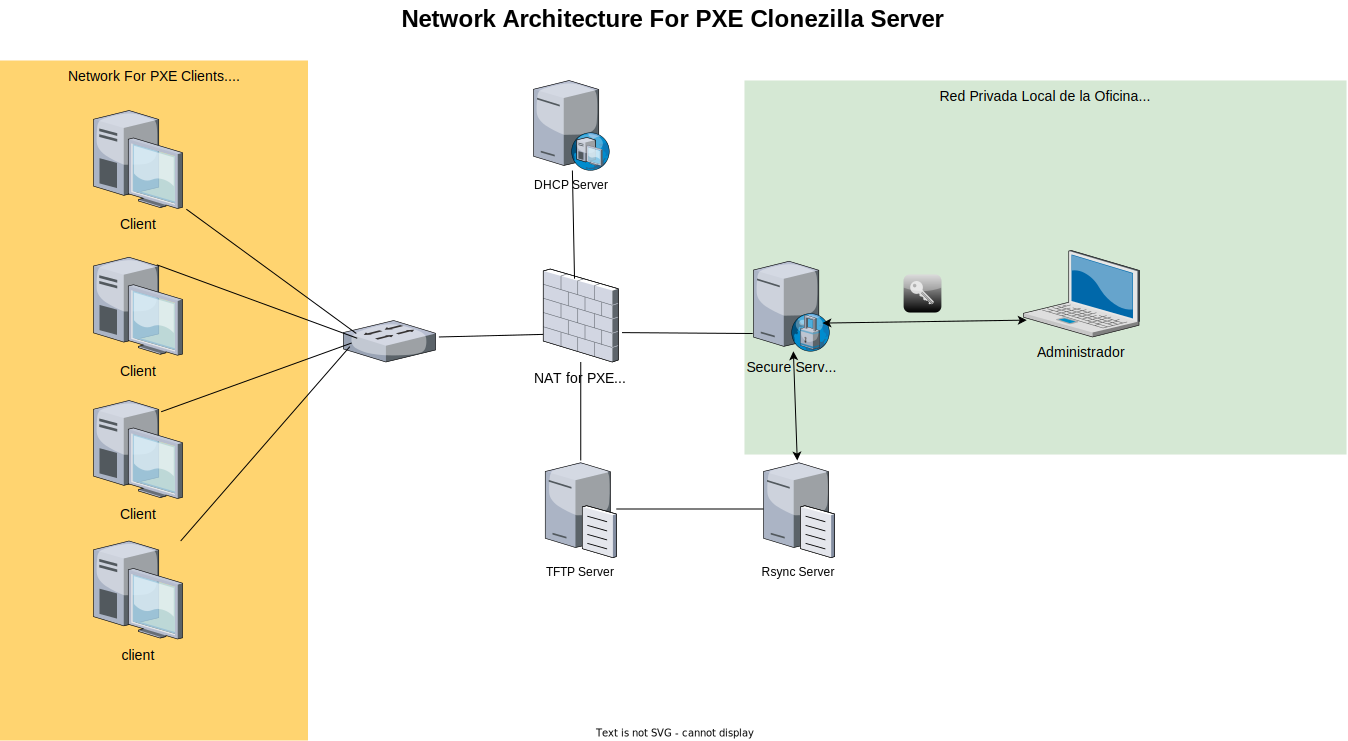
\includegraphics[scale=0.30]{drbl/network_diagram}
	\caption{Podemos ver los diversos servicios qu enecesita DRBL para poder trabajar así como los tipos de conexión establecida y la NAT que tiene.}
\end{figure}

Ahora explicamos las partes del playbook que debemos modificar para poder desplegar el servicio:

La primera parte consiste en que debemos poner la dirección IPv4 de la red de la oficina del servicio correcta, tiene que ser la misma que la que tiene asignada por DHCPv4 por el router o manualmente
si lo hemos hecho así. También debemos incluir la información de la puerta de enlace, el motivo por el que hacemos esto, es que el playbook desde las líneas 16 a 26 genera a partir
del fichero \textbf{templates/interfaces.j2}, un fichero en \textbf{/etc/interfaces}, con las variables arriba referidas, incluyendo la variable LAN que también puede ser tocada pero
necesitaría de una modificación adicional en el siguiente fichero \textbf{templates/drblpush.conf}, el motivo es porque dicha variable, al variar necesitas vigilar si el rango de direcciones
ip es el bueno para tu subred nueva, entonces la sección que debemos mirar son las líneas 40 a 47 ya que esas líneas son esenciales para un despliegue correcto del servicio DHCPv4 automatizado.


\begin{lstlisting}[style=mybash]
	vars:
    # DANGEROUS: Your WAN IP need to be the same if already as asigned to DHCP or Ansible did not auto reconnect
    iface_wan:
      - 192.168.122.68
    iface_wan_gateway:
      - 192.168.122.1
    iface_wan_nameservers:
      - 1.1.1.1
    iface_lan:
      - 192.168.111.1
\end{lstlisting}

Si cambiamos algún parámetro anterior, debemos de ir además al fichero de inventory.yml de la carpeta raíz ya que debemos ajustar las direcciones IPv4 y los hosts de manera acorde. En concreto
en ese fichero debemos poner el \textbf{ansible\_host: 192.168.122.68} igual que la interface\_wan. Si modificamos algo de iface\_wan debemos ir además al fichero de drblpush.conf.j2 y 
también al inventory.yml de la subcarpeta client\_ssh\_proxy ya que  tenemos que poner la dirección ssh del servidor en la siguiente variable de ssh y en la del host igual que en el inventory.yml de provisionamiento.

\begin{lstlisting}[style=mybash]
ansible_ssh_common_args: "-o ProxyCommand=\"ssh clonezilla@192.168.122.68 -o Port=22 -W %h:%p\""
\end{lstlisting}

La ejecución es totalmente automática con el siguiente comando, ask-become-pass te pide la contraseña para usar sudo o elevación de privilegios:
\begin{lstlisting}[style=mybash]
ansible-playbook --ask-become-pass playbooks/deploy_drbl.yml
\end{lstlisting}

Notas adicionales: En el momento de la edición del documento, el downgrade de grub aparentemente ya no hace falta, por lo que esa sección (líneas 80 85) están comentadas,
si se usa una versión antigua de Debian 11, descomentar dichas líneas para evitar la rotura de dependencias.

\newpage
\subsubsection{Proceso ilustrativo del despliege con ansible}

Una vez ejecutado el playbook y puesta la contraseña de sudo (become). La primera parte del playbook, indica si encuentra al servidor, rehará la configuración de red y reiniciará 
el servicio de red para poder aplicar los cambios. Si la tarea de reconnect no sigue adelante, es que ha fallado algo relacionado con la configuración de red, puede ser normalmente
por las configuraciones de variables de ip\_wan, que difiere con la ip real de reconexión del inventario.

\begin{figure}[H]
	\centering
	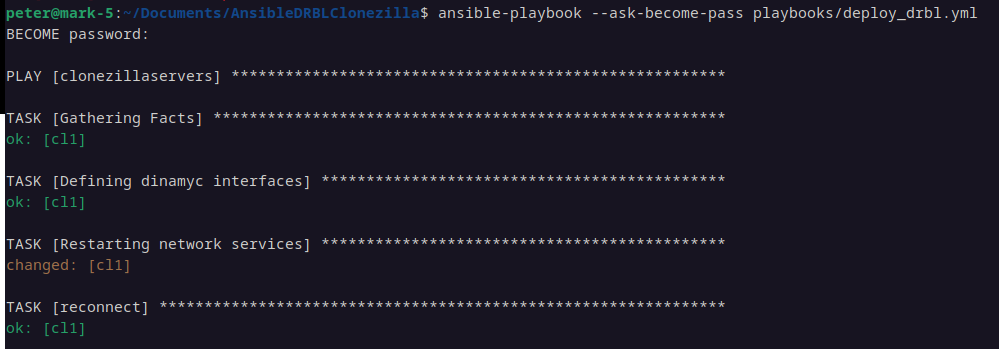
\includegraphics[scale=0.30]{deploy-drbl/deploy01}
	\caption{En esta sección el playbook indicara problemas de conectividad.}
\end{figure}

Luego a continuación, se puede observar el proceso de instalación de dependencias, que no es necesario reflejarlo en el libro ya que si ocurre algún fallo Ansible automáticamente
lo indicará, pero lo que si es clave, es que la siguiente tarea se complete bien observando el log antes de continuar, lo pondrá claramente gracias a la salida que se ha generado
con el playbook. El proceso es muy largo, ya que la configuración es decargar las dependencias necesarias de todos los subservicios dependientes y además las imágenes de instalación por red (netinstall)

\begin{figure}[H]
	\centering
	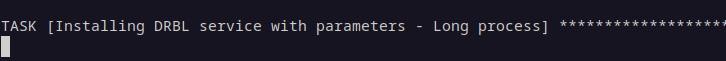
\includegraphics[scale=0.30]{deploy-drbl/deploy02}
	\caption{Tarea crucial para el correcto funcionamiento futuro del servicio.}
\end{figure}

\begin{figure}[H]
	\centering
	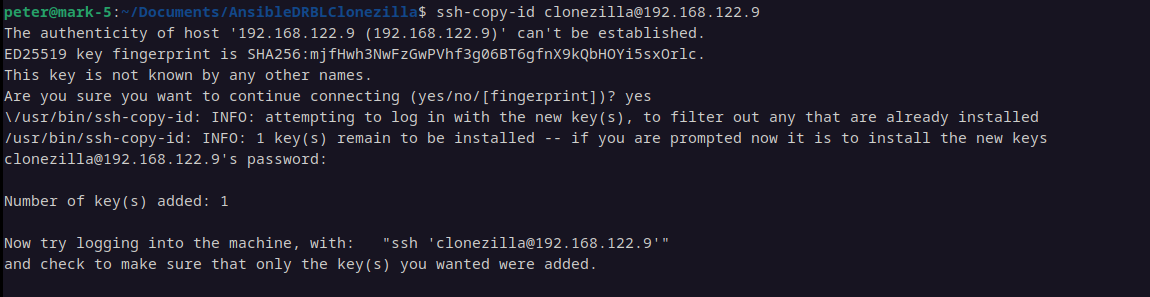
\includegraphics[scale=0.30]{deploy-drbl/deploy03}
	\caption{Si se ve la salida como en la ilustración es que todo ha ido bien y procede a realizar las configuraciones.}
\end{figure}

Las configuraciones de DRBL, son de manera resumida, los servicios DHCPv4, TFTP, de imagen, preparación de un kernel de arranque a partir del que tenemos, entre otros...

\begin{figure}[H]
	\centering
	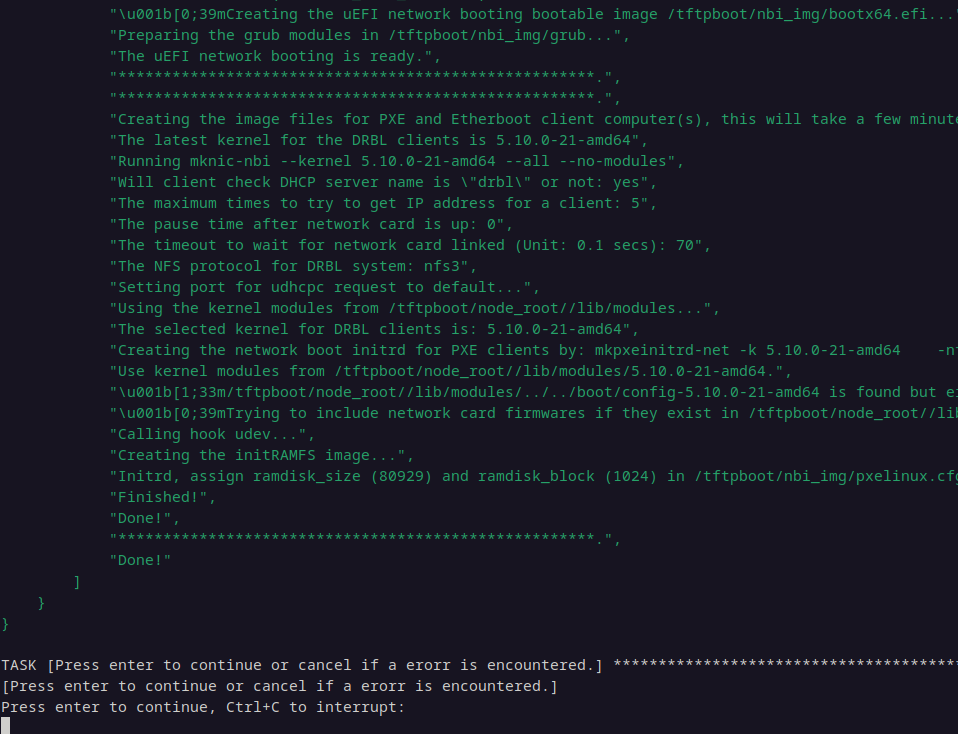
\includegraphics[scale=0.30]{deploy-drbl/deploy04}
	\caption{Si se ve la salida como en la ilustración es que todo ha ido bien y ya tenemos el servidor casi desplegado.}
\end{figure}

Ahora generará la configuración y nos indicará que ha ido todo bien tal y como sigue.

\begin{figure}[H]
	\centering
	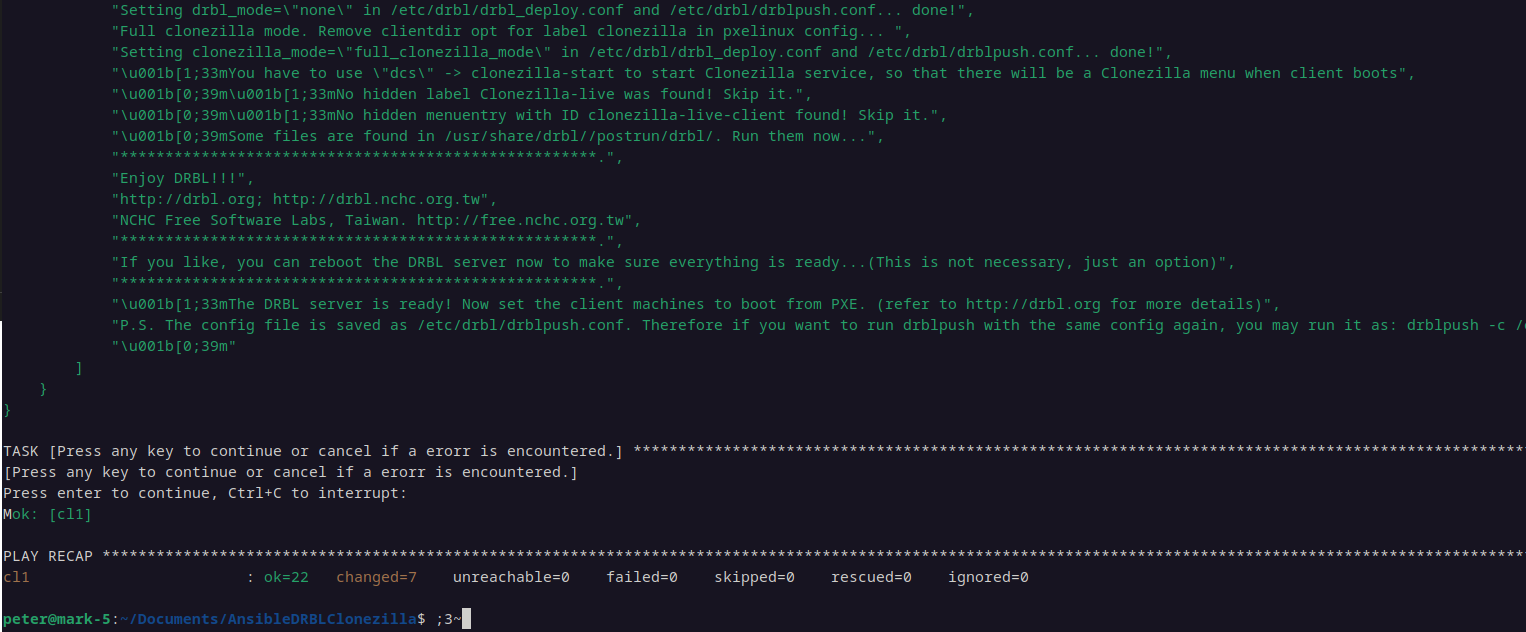
\includegraphics[scale=0.30]{deploy-drbl/deploy05}
	\caption{Si se ve la salida como en la ilustración es que todo ha ido bien y ya tenemos el servidor desplegado junto al resumen de Ansible.}
\end{figure}

\newpage
\subsection{playbook: provisioning\_ocs}

\textbf{Nota antes de instalar nada:} Debemos instalar rsync en nuestra workstation.

Este playbook se encarga de automatizar el proceso de subir la imagen en el directorio /home/partimag, que es donde el servicio DRBL lee para poder preparar la imagen para servirla
mediante PXE. La subida de la imagen se realiza mediante Rsync con varias comprobaciones de SHA (Hash) para comprobar que se han subido de manera correcta al servidor.
\vspace{5mm}
El playbook también incluye variables de control (yes/no) que permite controla qué queremos realizar con el, en concreto activa y desactiva las siguientes secciones:

\begin{itemize}
	\item Subida de imagen nueva *toda la carpeta.
	\item \textbf{Modo UNICAST}: Útil para cuando no queremos esperar a que haya un nº de máquinas prefijado o no las tengamos disponibles en estos momentos si no que va lanzando el programa 
	a cada máquina que lo solicite por PXE sin importar como vayan las demás máquinas. Este modo quizás sobrecargue más el servidor, ya que la demanda de los PCs en distintos tiempos en los que se encuentra
	puede generar una latencia de E/S importante junto al ancho de banda. Pero debido a que el servidor normalmente es más potente.
	\item \textbf{Modo MULTICAST}: Al contrario que en el modo anterior, espera dos tipos de variables, el tiempo de espera desde que el primer equipo se conecta y/o el nº de equipos
	que Clonezilla debe esperar para ejecutarse. Si lo ponemos de manera combinada, prevalece el tiempo de espera normalmente, si no te da tiempo a conectar la cantidad de PCs indicada 
	en este modo.
	\begin{itemize}
		\item Espera de un Nº de equipos: Ponemos un nº acorde de equipos sobre los cuales se va a lanzar el proceso de copia en MULTICAST. Máximo 18 por el límite de DHCPv4.
		\item Espera de segundos: Ponemos un número predeterminado de segundos que indique cuánto tiempo espera el servicio desde la primera solicitud de PXE.
		\item Modo combinado anterior: Se indican las dos variables anteriores, prevalece la que se cumpla antes, es decir si conectamos todos los equipos a tiempo antes de que cumpla dicho tiempo arranca el programa y en caso contrario se inicia el Multicast con los que haya, 
		siempre que se haya conectado primeramente un equipo por PXE. Este es el modo en el que está configurado el Ansible, ya que es el más eficiente.
	\end{itemize}
\end{itemize}

La parte de la imagen en concreto debemos tener obligatoriamente imagen\_name correctamente, ya que aunque no subamos una imagen, el playbook debe conocer cuál es su nombre 
para poder obtenerlo desde /home/partimag, en caso conctrario se termina la ejecución del playbook.
\vspace{5mm}

La parte de imagen\_origin es necesaria, ya que es una ruta local, absoluta o relativa, de nuestra workstation, donde tenemos la carpeta con los ficheros necesarios para realizar el proceso
de clonado. La transferencia se realiza por rsync, el playbooks se encarga de resolver dependencias de rsync si este no está disponible en el servidor (líneas 46 a 59) y en la máquina local debemos instalarlo por nuestra cuenta. 
El proceso de copia se cancela automáticamente junto con todo el playbook, si la imagen indicada no existe en el equipo local, o se haya copiado mal en el servidor remoto. Indicando cuál es el paso 
que ha fallado mediante assertions.
\vspace{5mm}

image\_name se puede poner de dos formas, debemos comentar una o otra según lo que vayamos a utilizar, si usamos la segunda forma con split debemos asegurarnos de que ha obtenido
bien el nombre.
\vspace{5mm}

Para ejecutar el playbook debemos hacerlo como en el de despliegue del servicicio con (ask-become-pass te pide la contraseña para usar sudo o elevación de privilegios): 
\vspace{5mm}

La ejecución es totalmente automática con el siguiente comando:
\begin{lstlisting}[style=mybash]
ansible-playbook --ask-become-pass playbooks/provisioning_ocs.yml
\end{lstlisting}

\newpage
\subsubsection{Proceso ilustrativo de la subida de la imagen y la selección del modo}

Primero tenemos que tener en cuenta la ruta de la imagen, en el caso ilustrativo está en:

\begin{figure}[H]
	\centering
	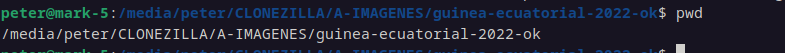
\includegraphics[scale=0.30]{provisioning-ocs/provisioning01}
	\caption{Ruta de la imagen absoluta que debemos poner en nuestra imagen.}
\end{figure}

Las variables que debemos tener en cuenta al principio del plabook, son:

\lstinputlisting[firstline=6,lastline=16,style=yaml]{../playbooks/provisioning_ocs.yml}

Explicación de las variables fijadas:

\begin{itemize}
	\item \textbf{push\_image} yes or no, activa el modo de rsync, util si no tienes la imagen instalada en el servidor. 
	\item \textbf{image\_origin} Indicamos la ruta absoluta o relativa de la ubicación de la carpeta de la imagen.
	\item \textbf{image\_name} Aquí podemos usar las dos formas, una con split (con comprobador de si lo has realizado bien) o poniendo el nombre de la imagen a mano.
	\item \textbf{workstation\_username} Nombre de usuario que usas actualmente en tu workstation local, necesario para comprobar que la ruta que has indicado como parámetro en push\_image existe.
	\item \textbf{clonezilla\_mode\_unicast} Se debe poner yes o no, es mutuamente excluyente con el modo multicast, si ponemos que sí en este modo el multicast se fija en no.
	\item \textbf{clonezilla\_mode\_multicast} Al ser mutuamente excluyente, no debemos modificar nada, solo que si ponemos no en el modo unnicast este modo se activa.
	\item \textbf{clonezilla\_mode\_multicast\_wait\_client} Variable que en la cual indicamos el n de clientes máximo que debemos esperar en este modo. Debemos tener en cuenta que DHCPv4 tiene un máximo de leases de 14
	\item \textbf{clonezilla\_mode\_multicast\_wait\_time} Variable en la cual indicamos la espera máxima (en segundos), desde que el primer cliente se conecta.
	\item \textbf{clonezilla\_disk\_restore} Variable a indicar dependiendo del nombre de la unidad clonada, puede ser sda, sdb,... Ver el final de esta sección para poder saber cuál es la correcta.
\end{itemize}

Proceso:

\begin{figure}[H]
	\centering
	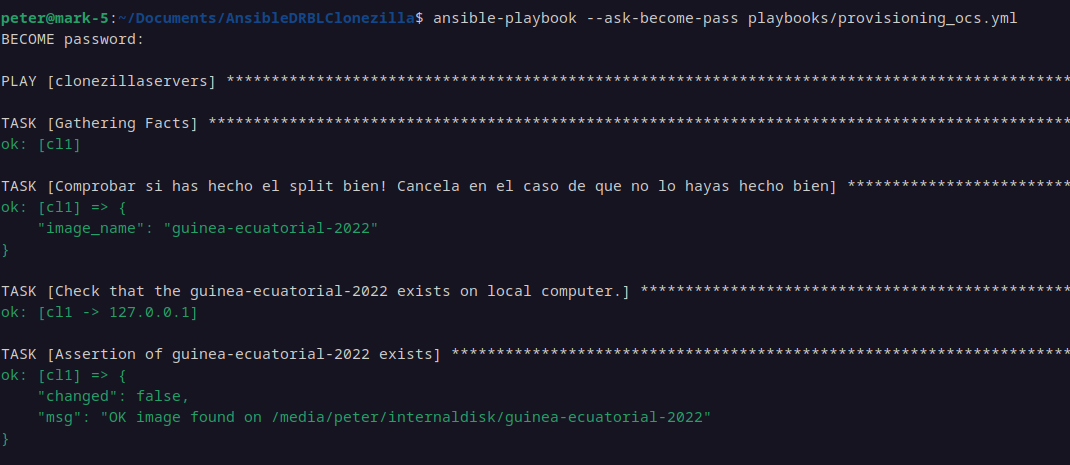
\includegraphics[scale=0.30]{provisioning-ocs/provisioning02}
	\caption{Proceso de copiado de la imagen y comprobación de que existe en el directorio de la workstation.}
\end{figure}

\begin{figure}[H]
	\centering
	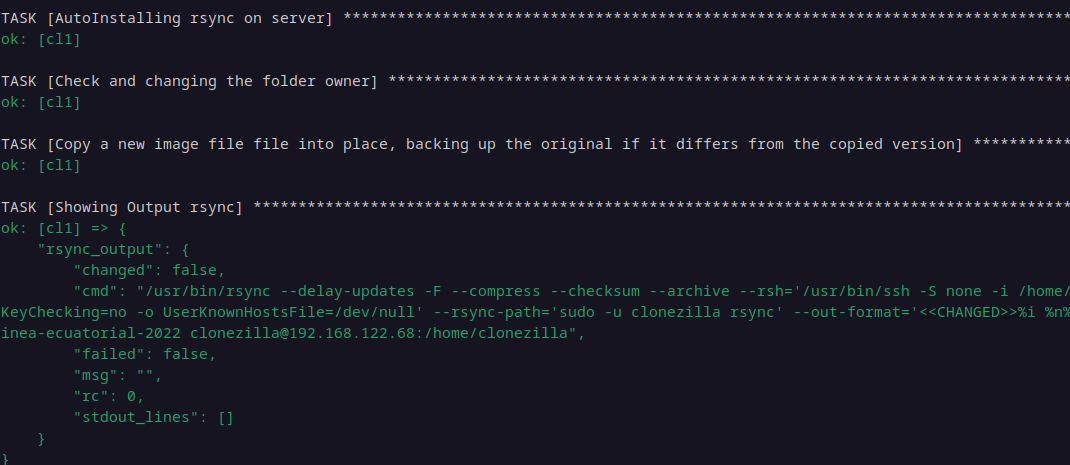
\includegraphics[scale=0.30]{provisioning-ocs/provisioning03}
	\caption{Proceso de instalación de rsync en el servidor y copiado de la carpeta con rsync.}
\end{figure}

\begin{figure}[H]
	\centering
	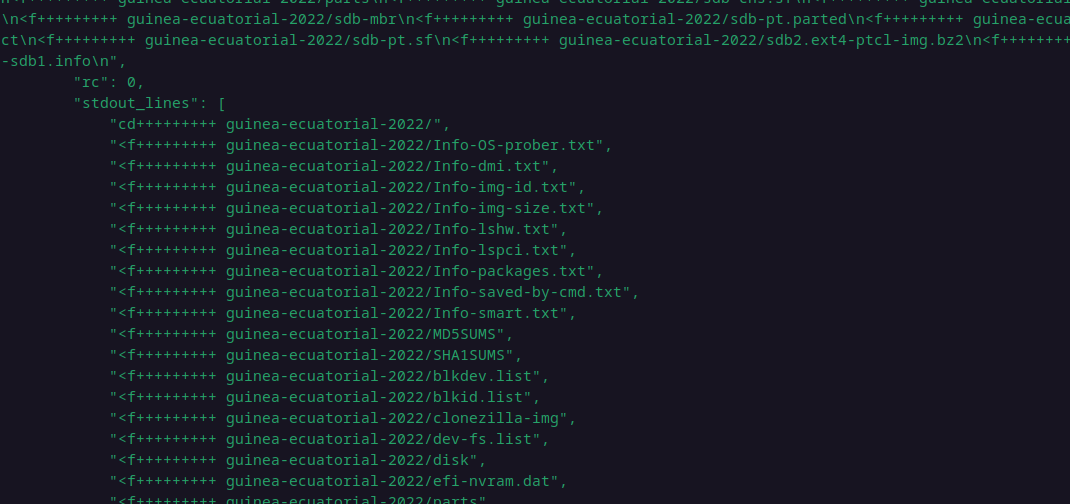
\includegraphics[scale=0.30]{provisioning-ocs/provisioning05}
	\caption{Rsync o synchronize te indica las diferencias si las hay.}
\end{figure}

\begin{figure}[H]
	\centering
	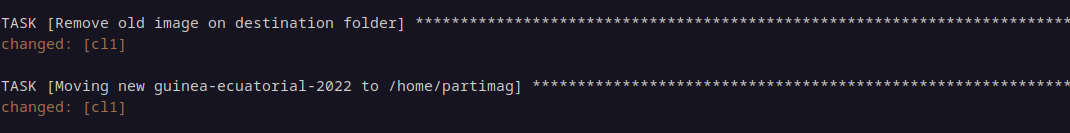
\includegraphics[scale=0.30]{provisioning-ocs/provisioning04}
	\caption{Proceso de eliminación de la carpeta antigua y moviendola a /home/partimag con los permisos adecuados.}
\end{figure}

\begin{figure}[H]
	\centering
	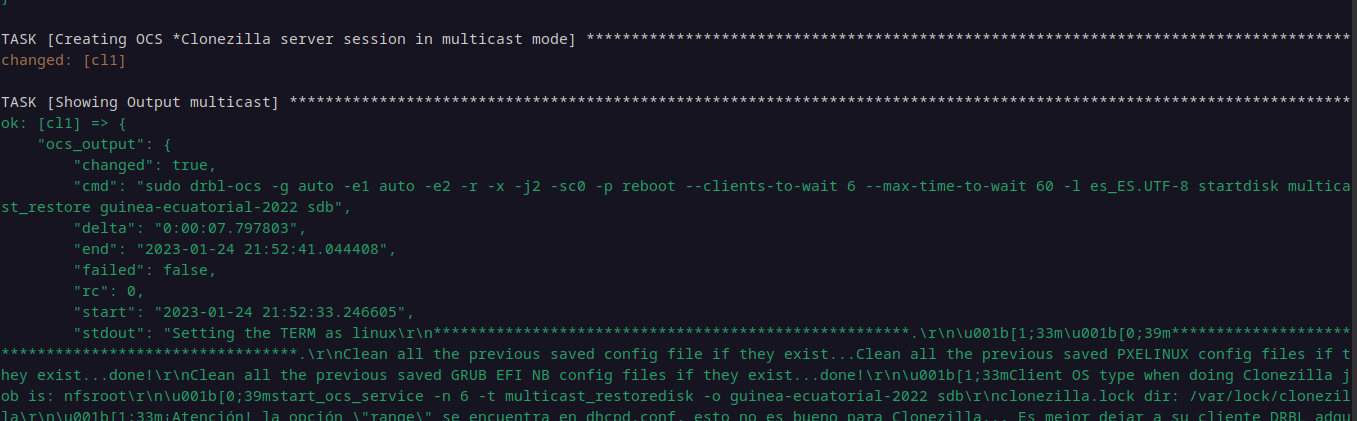
\includegraphics[scale=0.30]{provisioning-ocs/provisioning06}
	\caption{Modo MUTLICAST ejecutado correctamente.}
\end{figure}

\begin{figure}[H]
	\centering
	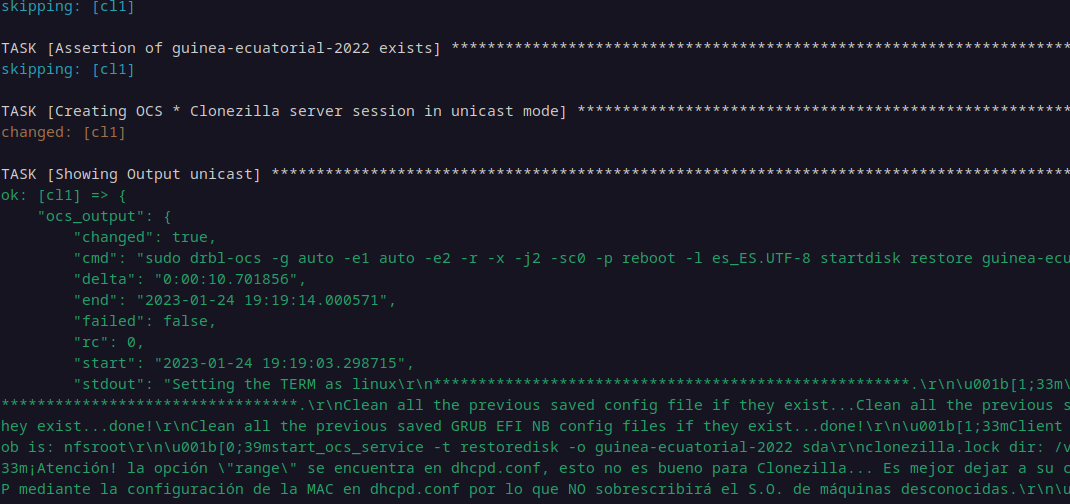
\includegraphics[scale=0.30]{provisioning-ocs/provisioning07}
	\caption{Modo UNICAST ejecutado correctamente.}
\end{figure}

Si alguna vez alguno de los dos modos no funciona correctamente o quiere realizar alguna otra operación como ejecutar un Memtest86+ o una imagen netinstall ejecute el siguiente comando:
\begin{lstlisting}[style=mybash]
sudo dcs	
\end{lstlisting}

\newpage
\subsubsection{Los modos no se ejecutan correctamente indicando que hay un problema con el disco/partición}

Si falla alguno de los dos modos indicando que el nombre del disco no es el correcto porque sea distinto a sda (como por ejemplos sdb o cualquier otro). Debemos 
ir a la ruta del directorio en /home/partimag/carpetaimagen, para ejecutar el siguiente comando y visualizar los binarios comprimidos que tengan la imagen, 
como en la imagen, se puede ver que es sdb en vez de sda, esto ocurre cuando hay más de un disco usado en el sistema clonado, debemos estar pendiente de esto.
\vspace{5mm}

\begin{figure}[H]
	\centering
	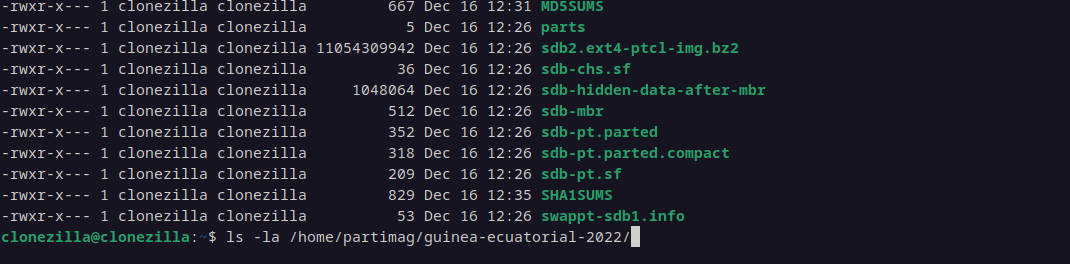
\includegraphics[scale=0.30]{provisioning-ocs/provisioning08}
	\caption{Buscando el nombre del disco que queremos recuperar correcto.}
\end{figure}

\begin{figure}[H]
	\centering
	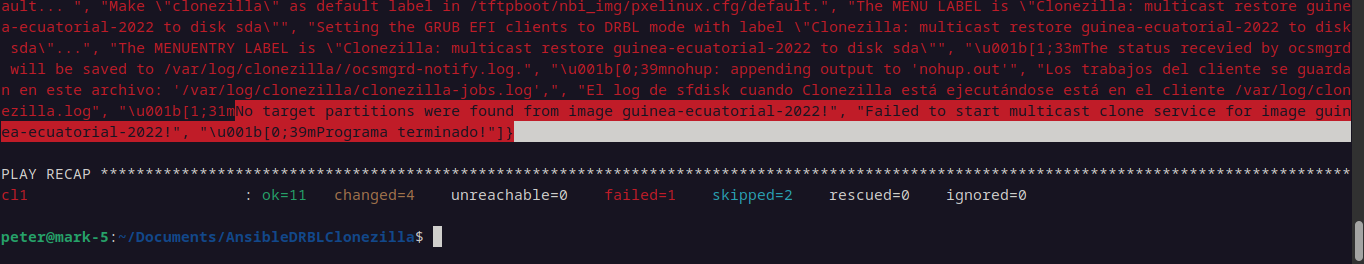
\includegraphics[scale=0.30]{provisioning-ocs/provisioning09}
	\caption{Identificación del error de los discos.}
\end{figure}

\begin{figure}[H]
	\centering
	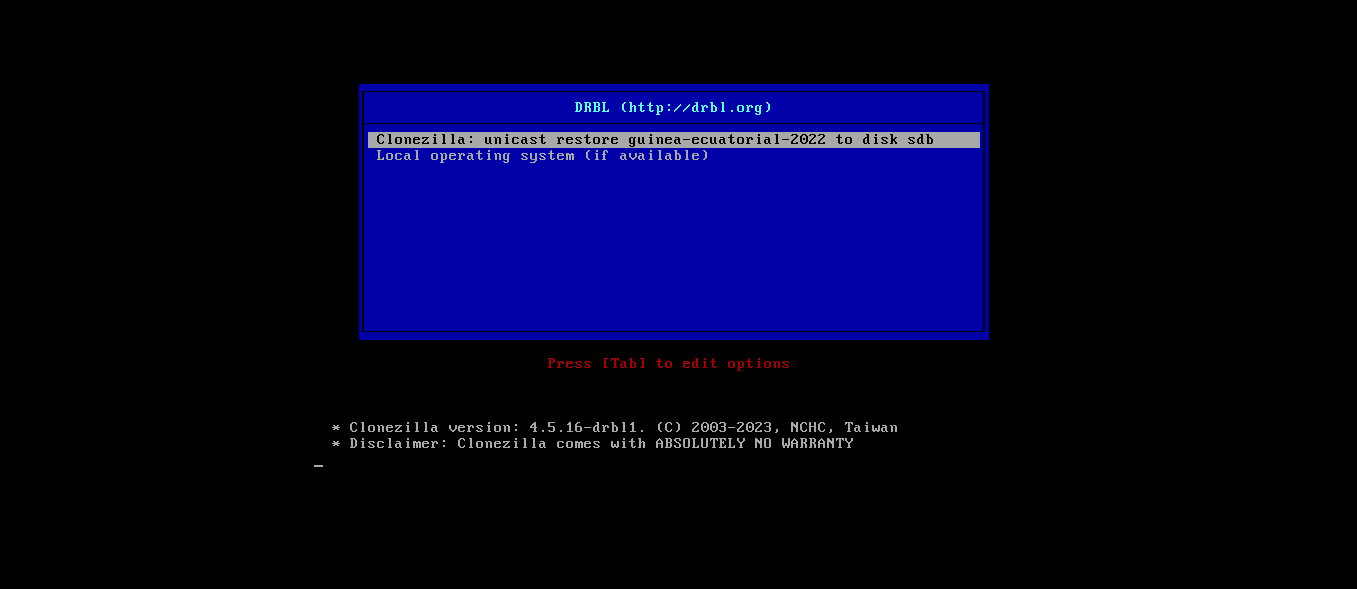
\includegraphics[scale=0.30]{provisioning-ocs/provisioning10}
	\caption{Cliente que ha recibido respuesta a la solicitud PXE del servidor.}
\end{figure}

\newpage
\subsection{playbook: update\_clients}

Esta necesidad es diferente a lo exigido antes, se parte de la necesidad de tener un método de actualización eficaz que no implique tener que ir al equipo físico
ya que implica una pérdida de tiempo en el que lo dedicamos a conectar el equipo a un monitor y teclado para poder realizar las actualizaciones. 
\vspace{5mm}
La solución ha sido configurar Ansible, en otra subcarpeta llamada \textbf{client\_ssh\_proxy}, otro inventario totalmente distinto que contiene la dirección IPv4 de cada
host cedida por lease con DHCPv4. Para poder usar un ssh bastion o jump, que implica usar al servidor donde está DRBL, como intermediario para saltar a los otros equipos clonados ya que
están dentrás de una NAT, por motivos de aislar las peticiones PXE.
\vspace{5mm}
Como pre-requisito clave, debemos tener la clave pública de nuestra workstation copiada dentro de la imagen y el servidor ssh. Así como cambiar el nombre de usuario de los hosts
clonados al que corresponda en su inventory.yml de la subcarpeta.

\begin{figure}[H]
	\centering
	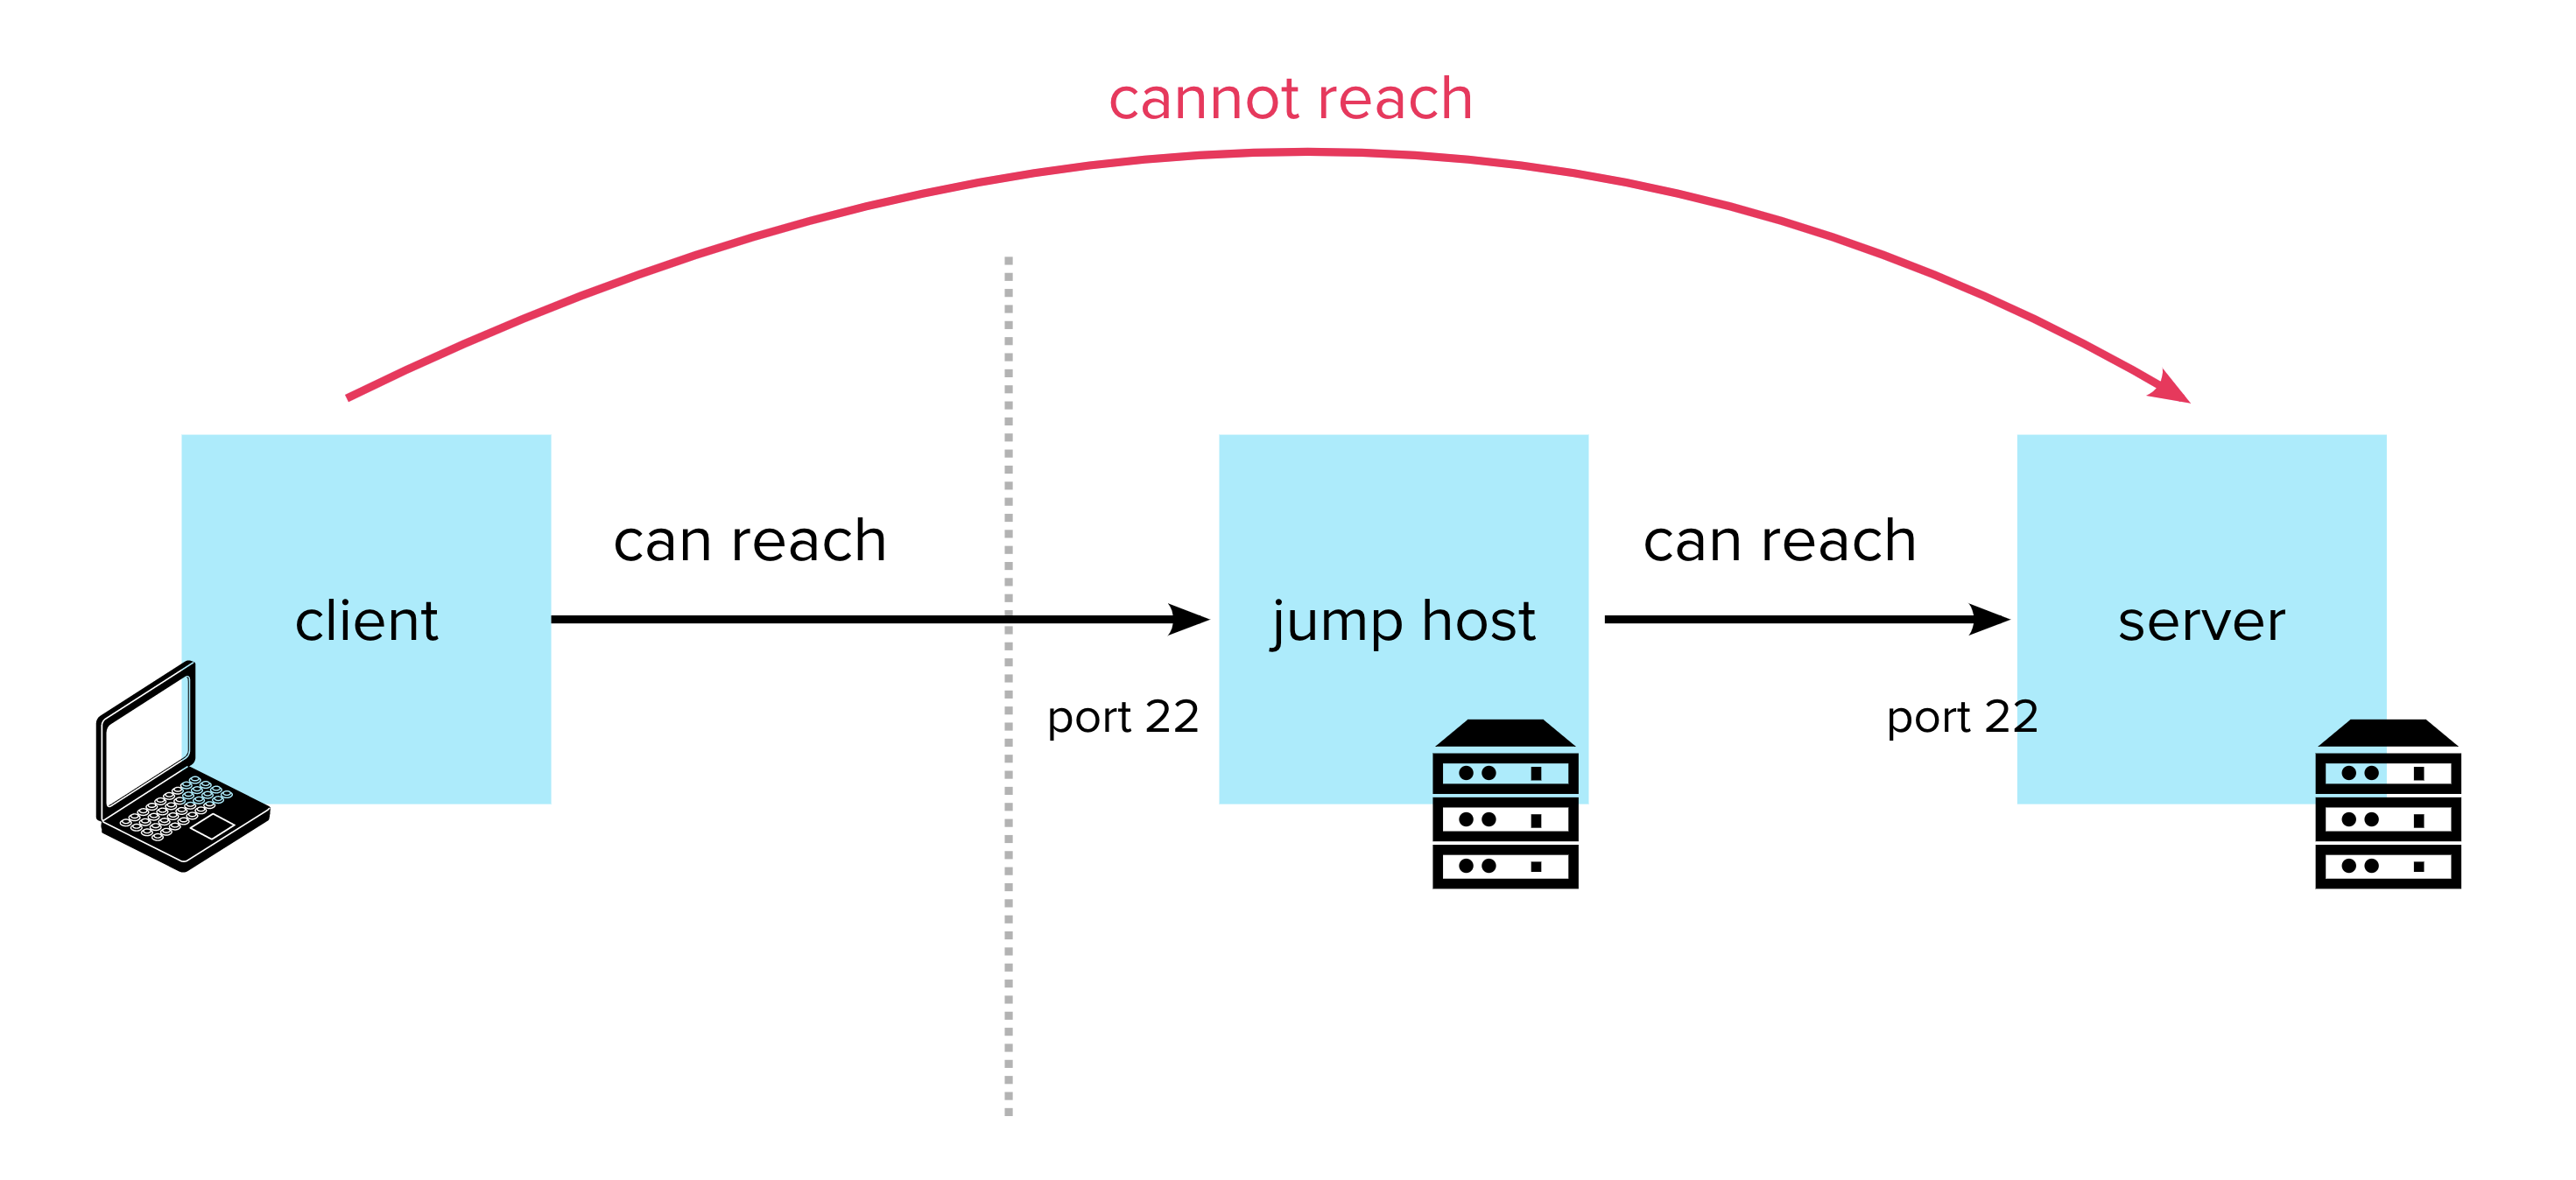
\includegraphics[scale=0.10]{update-clients/bastion.png}
	\caption{Funcionamiento de un servidor ssh bastión que se proporciona como punto de salto hacia otros hosts de ssh.}
\end{figure}

El playbook es sencillo implica la ejecución de un script previamente preparado para ser lanzado en contra de todos los clientes que haya detrás de la NAT de Clonezilla.

\lstinputlisting[style=yaml]{../client_ssh_proxy/playbook/update_clients.yml}

El script deberá estar correctamente escrito o comprobado, o en otro caso usar las utilidades de Ansible para provisionar a los clientes. Los scripts deben estar ubicados 
con un nombre único en la subcarpeta scripts.

\newpage
Como ejemplo de sustitución de los scripts de bash mejor controlados ponemos un ejemplo:

\lstinputlisting[style=yaml]{../client_ssh_proxy/playbook/update_clients_ansible.yml}

\newpage
\section{Anexo: SSH}

Generar nuestro id\_rsa básico, para poder utilizar Ansible, ya que depende del uso de las claves públicas para poder ejecutar todos los playbooks.

\begin{lstlisting}[style=mybash]
ssh-keygen
\end{lstlisting}

Para copiar nuestro id\_rsa.pub al servidor nuevo antes de la ejecución de los playbook y si queremos usar el módulo de actualizaciones de software también tenemos que 
hacerlo en la imagen que queramos clonar, pero este proceso será manual o distinto ya que la imagen se crea en un entorno aislado normalmente.

\begin{lstlisting}[style=mybash]
ssh-copy-id clonezilla@192.168.1.101
\end{lstlisting}

\begin{figure}[H]
	\centering
	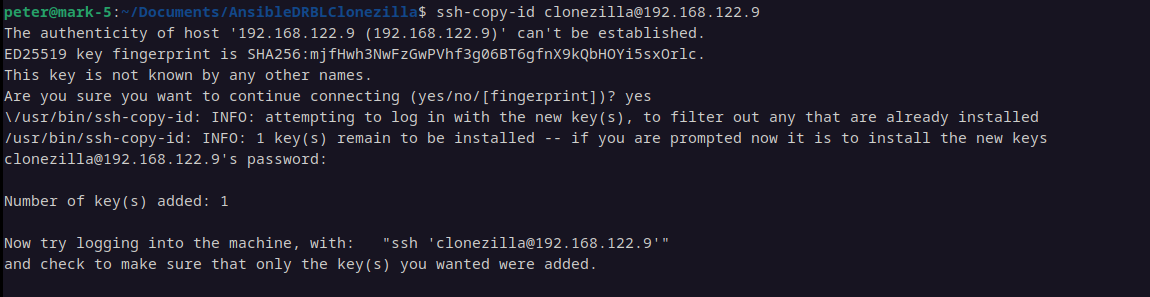
\includegraphics[scale=0.30]{anexo/copy-id}
	\caption{Proceso de copia de clave pública RSA al servidor..}
\end{figure}
	


% \vspace{5mm}


% \begin{lstlisting}[style=mybash]
%     # Para una base de datos concreta
%     mysqldump --user=tiendabd --password=password --databases tiendabd --add-drop-database --add-drop-table [--replace] --host=127.0.0.1 --result-file=dump.sql
% \end{lstlisting}



%\begin{figure}[H]
%	\centering
%	\includegraphics[scale=0.30]{cuestion_1_1}
%	\caption{Se puede ver que al no haber un fallo grave, el sistema lo nota como que sigue funcionando pero en un estado degradado.}
%\end{figure}

%\newpage

%Se pueden hacer include en latex
%\newpage

\section{Section}

\subsection{Subseccion}

\subsubsection{Subseccion}



%-------Bibliografia-----------------------------

%\newpage
\section{Bibliografía}

% Ejemplo
\footnote{Administración de mdadm - Por Red Hat}
\textcolor{blue}{\url{https://access.redhat.com/documentation/en-us/red_hat_enterprise_linux/8/html/managing_storage_devices/managing-raid_managing-storage-devices#monitoring-raid_managing-raid}}



\end{document}
